\documentclass[a4paper,9pt,twocolumn,twoside,]{pinp}

%% Some pieces required from the pandoc template
\providecommand{\tightlist}{%
  \setlength{\itemsep}{0pt}\setlength{\parskip}{0pt}}

% Use the lineno option to display guide line numbers if required.
% Note that the use of elements such as single-column equations
% may affect the guide line number alignment.

\usepackage[T1]{fontenc}
\usepackage[utf8]{inputenc}

% pinp change: the geometry package layout settings need to be set here, not in pinp.cls
\geometry{layoutsize={0.95588\paperwidth,0.98864\paperheight},%
  layouthoffset=0.02206\paperwidth, layoutvoffset=0.00568\paperheight}

\definecolor{pinpblue}{HTML}{185FAF}  % imagecolorpicker on blue for new R logo
\definecolor{pnasbluetext}{RGB}{101,0,0} %


\usepackage{booktabs}
\usepackage{longtable}
\usepackage{array}
\usepackage{multirow}
\usepackage{wrapfig}
\usepackage{float}
\usepackage{colortbl}
\usepackage{pdflscape}
\usepackage{tabu}
\usepackage{threeparttable}
\usepackage{threeparttablex}
\usepackage[normalem]{ulem}
\usepackage{makecell}
\usepackage{xcolor}

\title{Predicting the age of abalone by using only physical
measurements}

\author[a]{SIDs: 520420861}
\author[a]{520477636}
\author[a]{520556104}
\author[a]{500282597}
\author[a]{510041566}

  \affil[a]{DATA2002 Group 005E06, School of Mathematics and Statistics
Carslaw Building (F07) University of Sydney NSW 2006}

\setcounter{secnumdepth}{0}

% Please give the surname of the lead author for the running footer
\leadauthor{Group 005E06}

% Keywords are not mandatory, but authors are strongly encouraged to provide them. If provided, please include two to five keywords, separated by the pipe symbol, e.g:
 

\begin{abstract}
In this report, we aimed to predict the age of abalone from the
\href{https://archive.ics.uci.edu/dataset/1/abalone}{UCI Abalone
Dataset} by using only physical measurements. We found that a model
constructed using only the variables that can be measured from live
abalone was almost as accurate as the full model, and therefore
recommend that this model be used for future research endeavours, due to
its relative ease of use and animal welfare implications.
\end{abstract}

\dates{This version was compiled on \today} 


% initially we use doi so keep for backwards compatibility
% new name is doi_footer
\doifooter{\url{https://github.sydney.edu.au/yyeh7345/005E06}}

\pinpfootercontents{Group 005E06}

\begin{document}

% Optional adjustment to line up main text (after abstract) of first page with line numbers, when using both lineno and twocolumn options.
% You should only change this length when you've finalised the article contents.
\verticaladjustment{-2pt}

\maketitle
\thispagestyle{firststyle}
\ifthenelse{\boolean{shortarticle}}{\ifthenelse{\boolean{singlecolumn}}{\abscontentformatted}{\abscontent}}{}

% If your first paragraph (i.e. with the \dropcap) contains a list environment (quote, quotation, theorem, definition, enumerate, itemize...), the line after the list may have some extra indentation. If this is the case, add \parshape=0 to the end of the list environment.

\acknow{We used R version 4.3.1 \citep{RCoreTeam} to perform the
calculations, along with the \textbf{tidyverse} suite of packages,
including \textbf{ggplot2} for graphing \citep{tidyverse}. The
\textbf{gridExtra}, \textbf{cowplot}, \textbf{ggfortify},
\textbf{kableExtra} and \textbf{corrplot} packages were also used to
help produce the figures
\citep{gridExtra, cowplot, ggfortify, kableExtra, corrplot2021}.
Performance assessment was done using \textbf{caret} \citep{caret}. The
report was created using the `Pinp is not PNAS' template \citep{pinp}.}

\makeatletter
\let\oldlt\longtable
\let\endoldlt\endlongtable
\def\longtable{\@ifnextchar[\longtable@i \longtable@ii}
\def\longtable@i[#1]{\begin{figure}[t]
\onecolumn
\begin{minipage}{0.5\textwidth}
\oldlt[#1]
}
\def\longtable@ii{\begin{figure}[t]
\onecolumn
\begin{minipage}{0.5\textwidth}
\oldlt
}
\def\endlongtable{\endoldlt
\end{minipage}
\twocolumn
\end{figure}}
\makeatother

\hypertarget{introduction}{%
\section{Introduction}\label{introduction}}

The goal of our project was to predict the age of the abalone, or the
number of rings, by using physical measurements. This allows abalone to
be surveyed much more quickly. However, we still need to open up and
kill the abalone to measure the shucked, viscera and shell weight. This
partially defeats the purpose of predicting the number of rings since
the abalone still need to be killed.

As such, we produced a model that has access to all of the data,
alongside a live model that cannot use shucked, viscera and shell
weight. We found the best model for each data set and compared them to
assess if their performance is comparable. Based on this performance
assessment, we then made recommendations for the most optimal model for
surveying the age of abalone.

\hypertarget{data-set}{%
\section{Data set}\label{data-set}}

The data set consists of several physical measurements taken from a 4177
abalone of unknown origin. The majority of these are continuous
variables, except for sex, which is categorical, and rings, which is an
integer that provides the age of the abalone if we add 1.5. The rings
were counted by cutting and staining the abalone shell, before using a
microscope to inspect and count each of the rings \citep{abalone}. In
the original data, all of the continuous variables were divided by 200
so to simply result reporting, we reversed this by multiplying them by
200.

\hypertarget{analysis}{%
\section{Analysis}\label{analysis}}

The data set had no missing values and was assumed to be independent, as
long as no individual abalone were measured twice. The distribution of
rings is positively skewed.

\hypertarget{pre-modelling-assumption-checking}{%
\subsection{Pre-Modelling Assumption
Checking}\label{pre-modelling-assumption-checking}}

To meet the assumptions of a valid linear regression, the dependent and
independent variables must have a linear relationship including a
consistent variance. There should also not exist multicollinearity
amongst independent variables.

The variables were not linearly correlated with rings as the data fanned
out, while sex did not seem to significantly affect the distributions,
although infant abalone made up the bulk of the lower data points
(Figure 1).

To improve the linearity of these relationships, we scaled the variables
using the following scaling factors:

\(\log_{10}(\widehat{\text{Rings}}) = \beta_0 + \beta_a\text{Sex}[M] + \beta_b\text{Sex} [F] + \beta_c\text{Sex}[I] + \beta_1\log_{10}(\text{Length}) + \beta_2\log_{10}(\text{Diameter}) + \beta_3\text{Height} + \beta_4\log_{10}(\text{Whole Weight}) + \beta_5\log_{10}(\text{Shucked Weight}) + \beta_6\log_{10}(\text{Viscera Weight}) + \beta_7\log_{10}(\text{Shell Weight}) + \varepsilon_i\)

Figure 2 shows the improved linearity of the scaled data.\\

Multicollinearity may affect the usefulness of our model as all of the
variables are highly positively correlated, but none of the variables
were perfectly correlated (having a correlation coefficient of ±1), so
it was not a major concern (Figure 3).

\hypertarget{model-selection---original-model}{%
\subsection{Model Selection - Original
Model}\label{model-selection---original-model}}

To select the best variables as predictors for log rings, the following
analysis facilitates the AIC minimisation approach. The forward-stepping
method starts from the null model consisting of none of the variables in
the data set and adds the most formative variable in turn. In contrast,
the backward-stepping method starts from the full model consisting of
all variables in the data set and removes the least formative variables
from the model in turn. Both approaches aim to minimise the AIC value.

Both the forward and backward-stepping methods suggested that the full
model the the most optimal selection.

\hypertarget{model-assumption-checking---original-model}{%
\subsection{Model Assumption Checking - Original
Model}\label{model-assumption-checking---original-model}}

For a multiple regression model to be valid, the model has to satisfy
the following assumptions:

\begin{itemize}
\tightlist
\item
  Linearity: Residuals are approximately symmetrical in their
  distribution above and below zero.
\item
  Homoscedasticity: Residuals are scattered symmetrically around the 0
  line with fairly even variance and linearity.
\item
  Normality: Residuals are approximately normally distributed since most
  of the points align with the normal line in the QQ plot.
\end{itemize}

The residual and QQ plots (Figure 4) suggest that the assumptions are
not seriously violated. The residuals are mostly linearly and evenly
scattered, and the residuals mostly align with the theoretical quantile
line.

\hypertarget{a-more-context-logical-model---live-abalone}{%
\subsection{A More Context-Logical Model - Live
Abalone}\label{a-more-context-logical-model---live-abalone}}

While the model selection process is statistically based, the variables
selected should also make logical sense in the real-world context. The
shucked, viscera and shell weights can only be measured by killing and
opening the abalone. However, by opening an abalone, the number of rings
can be counted without the need for predictions. Therefore to improve
the usefulness of our model, the subsequent analysis will be carried out
using the `live' abalone data set, created by removing log shucked,
viscera and shell weights from the original scaled data set.

Another benefit associated with the live abalone model is a reduction in
redundant variables. Since shucked, viscera and shell weights all
contribute and a highly correlated with the whole weight, the model can
simply use the aggregate information, the whole weight, as the
predictor. This results in a decrease in multicollinearity, although the
correlation between the remaining variables may still hinder our model's
usefulness.

\newpage

\hypertarget{model-selection---live-abalone}{%
\subsection{Model Selection - Live
Abalone}\label{model-selection---live-abalone}}

The model selection approach for the live abalone data set replicates
that of the original scaled data set above, using the AIC minimisation
approach.

Again, both forward and backward-stepping methods suggested that the
full model of the live abalone data set is the most optimal selection.

\hypertarget{model-assumption-checking---live-abalone}{%
\subsection{Model Assumption Checking - Live
Abalone}\label{model-assumption-checking---live-abalone}}

Similarly to the original model, the live abalone model has to meet the
linearity, homoscedasticity and normality assumptions.

The residual and QQ plots (Figure 5) suggest that the assumptions are
not seriously violated. The residuals are mostly linearly and evenly
scattered, and the residuals mostly align with the theoretical quantile
line.

\hypertarget{results}{%
\section{Results}\label{results}}

\hypertarget{models-produced}{%
\subsection{Models Produced}\label{models-produced}}

The mathematical expressions of the original model is as follows:\\

\(\log_{10}(\widehat{\text{Rings}}) = 0.523 + 0.000446(\text{Sex}[F]) - 0.0226(\text{Sex}[I]) -0.315(\log_{10}(\text{Length})) + 0.201(\log_{10}(\text{Diameter})) + 0.000555(\text{Height}) + 0.59(\log_{10}(\text{Whole Weight})) -0.583(\log_{10}(\text{Shucked Weight})) -0.0759(\log_{10}(\text{Viscera Weight})) + 0.366(\log_{10}(\text{Shell Weight}))\)\\

Sex is an categorical variable, so replacing a sex with 1 and others
with 0 indicates the corresponding sex. The male sex has become the
intercept. The inferences of the model include:

\begin{itemize}
\tightlist
\item
  log-log relationships:

  \begin{itemize}
  \tightlist
  \item
    For every 1\% increase in Length, holding all else constant, the
    number of rings is expected to decrease by 0.315\%.
  \item
    For every 1\% increase in Diameter, holding all else constant, the
    number of rings is expected to increase by 0.201\%, etc.
  \end{itemize}
\item
  log-linear relationship:

  \begin{itemize}
  \tightlist
  \item
    For every 1 unit increase in Height, holding all else constant, the
    number of rings is expected to increase by 0.056\%.
  \end{itemize}
\end{itemize}

The mathematical expressions of the live abalone model is as follows:\\

\(\log_{10}(\widehat{\text{Rings}}) = 0.519 + 0.00480(\text{Sex}[F]) - 0.0355(\text{Sex}[I]) -0.580(\log_{10}(\text{Length})) + 0.649(\log_{10}(\text{Diameter})) + 0.00202(\text{Height}) + 0.163(\log_{10}(\text{Whole Weight}))\)\\

Sex is interpreted in the same manner as the original model, with 1 used
to indicate the corresponding sex and the male sex incorporated into the
intercept. The inferences of the model include:

\begin{itemize}
\tightlist
\item
  log-log relationships:

  \begin{itemize}
  \tightlist
  \item
    For every 1\% increase in Length, holding all else constant, the
    number of rings is expected to decrease by 0.580\%,
  \item
    For every 1\% increase in Diameter, holding all else constant, the
    number of rings is expected to increase by 0.649\%, etc.
  \end{itemize}
\item
  log-linear relationship:

  \begin{itemize}
  \tightlist
  \item
    For every 1 unit increase in Height, holding all else constant, the
    number of rings is expected to increase by 0.202\%.
  \end{itemize}
\end{itemize}

\hypertarget{performance-assessment}{%
\subsection{Performance Assessment}\label{performance-assessment}}

The performance assessment compares the in-sample and out-of-sample
performance of both the original and live abalone models.

The in-sample performance can be evaluated by comparing the \(r^2\)
value, which is the percentage of the variation of the dependent
variable that can be explained by that of the independent variables.
Thus, the greater the \(r^2\), the better the model at predicting values
that it has been trained on.

The out-of-sample performance was evaluated by looking at the RMSE and
MAE, both of which measure the error of prediction. This means that
smaller RMSE and MAE values correspond with better the out-of-sample
performance.

The assessment was carried out using repeated cross-validation, which
iteratively resamples training and test data sets to compare the
performance of the models and mitigate the impact of variation between
different samples.

The following results suggest that the original model, as expected, has
a better in-sample performance as it consists of more explanatory
variables than the live abalone model (\(r^2\): 0.638 \textgreater{}
0.504). Additionally, the original model also has a better out-of-sample
performance, having slightly lower RMSE and MAE than the live abalone
model.

\hfill\break
\textbf{Live Abalone Model: }\\

\begin{tabular}{r|r|r}
\hline
Rsquared & RMSE & MAE\\
\hline
0.504 & 0.098 & 0.075\\
\hline
\end{tabular}

\hfill\break
\textbf{Original Model: }\\

\begin{tabular}{r|r|r}
\hline
Rsquared & RMSE & MAE\\
\hline
0.638 & 0.084 & 0.064\\
\hline
\end{tabular}

\hypertarget{discussion-and-conclusion}{%
\section{Discussion and Conclusion}\label{discussion-and-conclusion}}

The original model offers limited performance gains but comes with
significant environmental consequences. This makes it more suitable for
surveying abalone already intended for consumption rather than research,
and emphasises the importance of balancing predictive accuracy and
environmental impact in model choice.

The live model uses a much less invasive method and improves animal
welfare, making it more socially acceptable. By requiring less
measurements, this method is also quicker and more cost-effective to
use. However, care must still be taken when returning the abalone, which
may be an additional cost consideration.

The model here does have a few limitations however. By scaling the
variables, we decreased the models' interpretability. This scaling also
led to very low coefficients, which are vulnerable to being affected by
minor rounding errors. Many of the variables also had correlation
between them, indicating multicollinearity and therefore some degree of
redundancy (Figure 3). AIC also has a tendency to overfit, although our
large sample size and small number of dimensions mitigates this concern
\citep{hurvich}.

The model may not be generalisable to other species of abalone, so the
model could be further improved by testing on other species of abalone
from other places in the world. Other models, such as neural networks,
may also be explored to see if they can achieve stronger correlation and
improved accuracy.

In conclusion, the non-invasive method offers similar accuracy while
favouring animal welfare and being easy to use, making it our model of
choice in real-world scenarios.

\newpage

\begin{figure}

{\centering 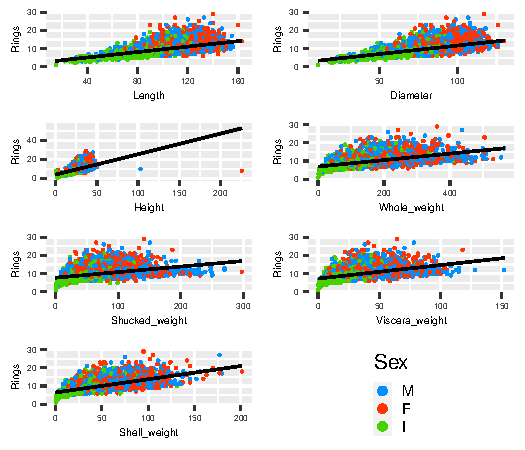
\includegraphics{005E06-Project-Report_files/figure-latex/original_scatter-1} 

}

\caption{Original data scatter plot, comparing independent variables with rings}\label{fig:original_scatter}
\end{figure}

\begin{figure}

{\centering 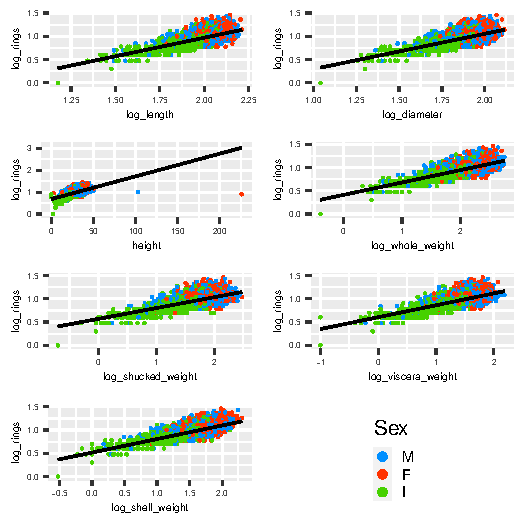
\includegraphics{005E06-Project-Report_files/figure-latex/scaled_scatter-1} 

}

\caption{Scaled data scatter plot, comparing independent variables with rings}\label{fig:scaled_scatter}
\end{figure}

\begin{figure}

{\centering 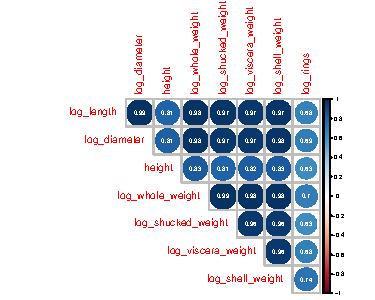
\includegraphics{005E06-Project-Report_files/figure-latex/correlation_matrix-1} 

}

\caption{Correlation heatmap (scaled)}\label{fig:correlation_matrix}
\end{figure}

\begin{figure}

{\centering 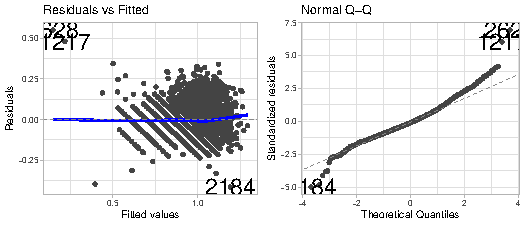
\includegraphics{005E06-Project-Report_files/figure-latex/original_assumptions-1} 

}

\caption{Original model residual and QQ plots}\label{fig:original_assumptions}
\end{figure}

\begin{figure}

{\centering 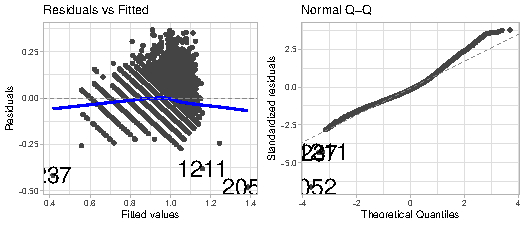
\includegraphics{005E06-Project-Report_files/figure-latex/live_assumptions-1} 

}

\caption{Live model residual and QQ plots}\label{fig:live_assumptions}
\end{figure}

%\showmatmethods
\showacknow


\bibliography{report}
\bibliographystyle{jss}



\end{document}
